\chapter{Фотопереключатели на основе гет(арил)стильбенов и краун-эфиров. ESIPT люминесценция (обзор литературы)} \label{chapt1}

	Среди большого разнообразия различных органических фотопереключателей особую роль играют фотопереключатели на стильбенах и их гетероциклических аналогах. Стильбены обладают как хорошей люминесценцией \cite{Krasovitsky_Bolotin}, так и способностью к высокоэффективному быстрому фотопереключению. Стильбены отличаются относительной простотой в получении \cite{Wood1941} и широкой возможностью для модификации функциональными заместителями и гетероциклическими фрагментами, что позволяет создавать структуры со сложным фотофизическим и фотохимическим поведением. \cite{Waldeck_D_H1991_Stilbenes} 
	
	Гетероциклические аналоги стильбенов позволяют улучшить люминесцентные свойства за счёт создания сопряжённой донорно-акцепторной пары. Наличие акцепторного азинового (азинонового) ядра в молекулах благодаря вкладу \textit{n},$\pi$*-состояния может оказывать заметное влияние на фотохимическое и фотофизическое поведение люминофоров. \cite{Lower1966} Азотсодержащие гетероциклические фрагменты, такие как пиримидин, хиназолин, хиноксилин и другие, зарекомендовали себя как хорошие акцепторные заместители, обладающие как собственной люминесценцией \cite{Krasovitsky_Bolotin}, так и работающие в паре с арильными донорами.
	
	Краун-содержащие гет(арил)стильбены хорошо представлены в литературе \cite{Gromov_2006_Crowns_in_Stilbenes}. В основном, краун или бензокраунсодержащий фрагмент является частью стильбена. 

	\section{Синтез, фотофизические и фотохимические свойства гетероциклических аналогов стильбенов}\label{sect1_1}
	
		\subsection{Синтез}
	
			Текст первой главы
		
			\begin{figure}
				\centering
				\caption{Стильбен}
				\label{fig:stilbene}
				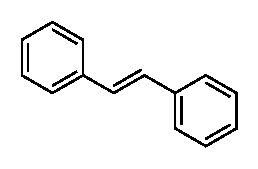
\includegraphics{Dissertation/images/part1/Stilbene}
			\end{figure}
			
			